
Benchmark-based evaluation is often used to predict the effect of a set of code transformations on the performance of actual applications that resemble the benchmark used in the evaluation. An issue with many of the performance evaluations of \FDO-based code transformations published in the literature is the lack of exploration of the effect of different data input on the reported results. An interesting question is how misleading a performance prediction that uses a single data input may be.

The goal of this section is to investigate the potential error in the prediction for the case of \FDI\ using combined profiling. The following experiment compares an \FDI\ with the standard inliner from \llvm: (1) Select a reasonable set of data inputs for a given benchmark; (2) Execute all combinations of single-input profiling/single-input testing for the \FDO\ inliners, repeating each test run a number of times that is sufficient to capture runtime variances;\footnote{For the experiments described in this paper an empirical statistical study using 1000 runs revealed that three runs were sufficient.}  (3) Run the \llvm\ inliner on all inputs --- the same number of times as in (2) for each input; (4) To illustrate the best performance of \FDI\ that could be reported from the data, select the best run amongst all profiling/testing combinations for a given test input and compare with the worst run for the \llvm\ inliner; (5) To demonstrate the worst performance of \FDI, do the opposite, look for the worst \FDI\ run and the best \llvm\ run for a given test input; (6) To find what the actual comparison is, use all but the test input to generate a combined profile and use this combined profile in \FDI; (7) execute this binary the necessary number of times and compare the average of these runs with the average of the same number of runs using the \llvm\ inliner.

\begin{figure*}
\begin{center}
  \subfigure[\FDI\ is faster than \llvm;]{
    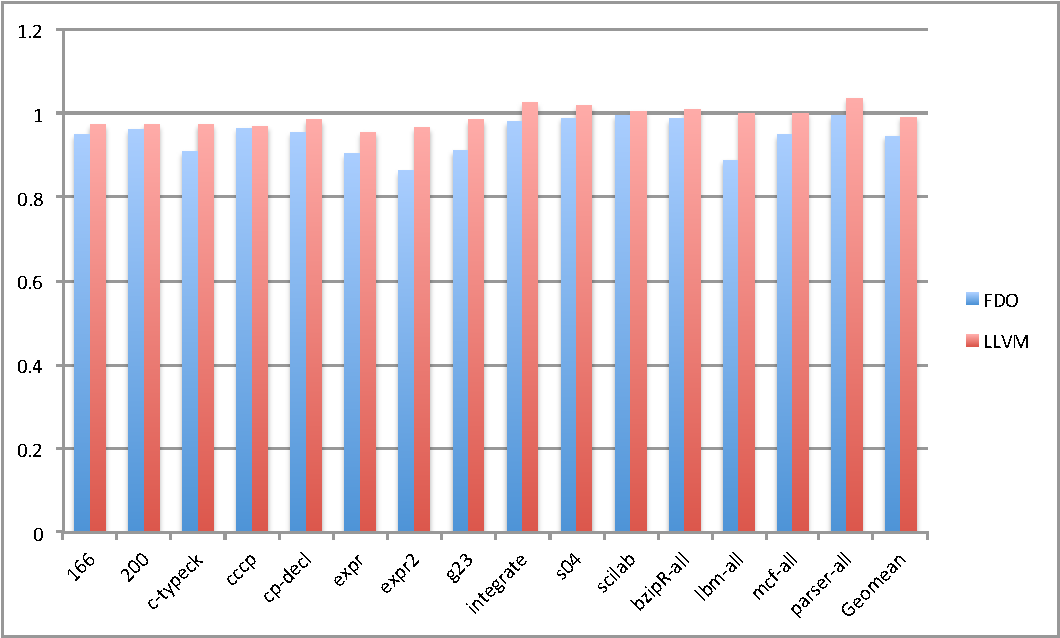
\includegraphics[width=0.4\linewidth]{Figures/speedupgccall}
     \label{fig:BestFDIWorstLLVMgcc}
  }
 \subfigure[\FDI\ is slower than \llvm;]{
    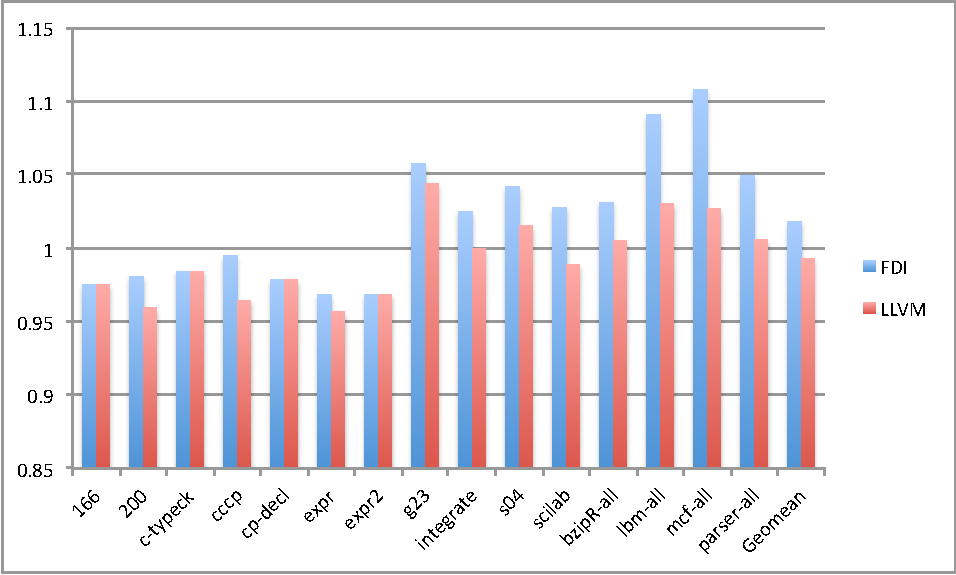
\includegraphics[width=0.4\linewidth]{Figures/slowdowngccall}
     \label{fig:WorstFDIBestLLVMgcc}
  }
  \end{center}
 \caption{Performance Study for \gcc. (a) Best runs of \FDI\ compared with worst runs of \llvm.  (b) Worst runs of \FDI\ compared with best runs of \llvm. Bar heights represent running time normalized to running time of Never}
  \label{fig:BestWorstComparison}
\end{figure*}

This performance evaluation uses an infrastructure based on the \llvm\ development framework. This infrastructure includes a set of C++ programs and a set of scripts to control the machine-learning training, the compilation and the execution of performance runs. This single infrastructure offers the option of performing both single-run-training/single-run-testing \FDO\ and  \CP-based \FDO\ with multiple-run performance evaluation. The number of runs used for \CP\ and for the evaluation are parameters set by the experimenter~\cite{BerubePhD}.

%======== Setting: machines, inputs, describe

The experiments were conducted on $20$ Dell Optiplex 755 running Slackware Linux 2.6.32.39 each equipped with Intel Duo Core E6750 2.66 GHz processors, 4 GB RAM, DVD-RW drive, Intel Pro/1000 Gb ethernet, Gigabyte GeForce 8600 video cards, and 250 GB SATA II drive. 

\subsection {Experimental Results}

The first case study uses the SPEC CPU 2006  \gcc\ evaluated with fifteen inputs. The eleven inputs distributed with SPEC CPU 2006 are augmented with  four SPEC 2000 benchmark programs used as input: \bzip, \lbm, \mcf, and \parser. To be used as inputs these programs had to be converted to the single pre-processed file format required by the \gcc\ benchmark.
Figure~\ref{fig:BestWorstComparison}  presents the result of the comparison between \llvm and \FDI. The objective of this figure is to illustrate how an experimental evaluation that performs a single execution can result in misleading results and conclusions. For each test input the \FDI\ measurement uses a leave-one-in methodology where all inputs, except the one used for testing, are used for training. is and \llvm. The baseline for comparison is  {\tt Never} which is a version of the compiler that uses an inlining cost function that limits inlining to callers containing a single basic block and that are expected to increase the code size in the caller by at most three instructions~\cite{BerubePhD}.

For all runs on individual inputs for a given version of the compiler, the reported execution time is the minimum of the execution time of three runs. This measuring method is selected to minimize interference from machine activity, such as network transactions or operating system interrupts, that are unrelated with the inlining strategy under study.  Each bar in Figure~\ref{fig:BestWorstComparison} is the result of comparing the time obtained in a single execution. These results indicate the range of performance that could be reported by a careless experimental evaluation that uses a single execution of each version to report performance variations. The conclusion could vary from saying that \FDI\ is 2.4\% faster than \llvm\ to saying that \llvm\ is 2.8\% faster than \FDI. What is the true relative performance between the two versions? The next section provides a description of the Combined Profiling methodology that will be used to determine the actual performance comparison between \FDI\ and \llvm.
 
\REM{
\begin{figure*}
\begin{center}
  \subfigure[\FDI\ is faster than \llvm;]{
    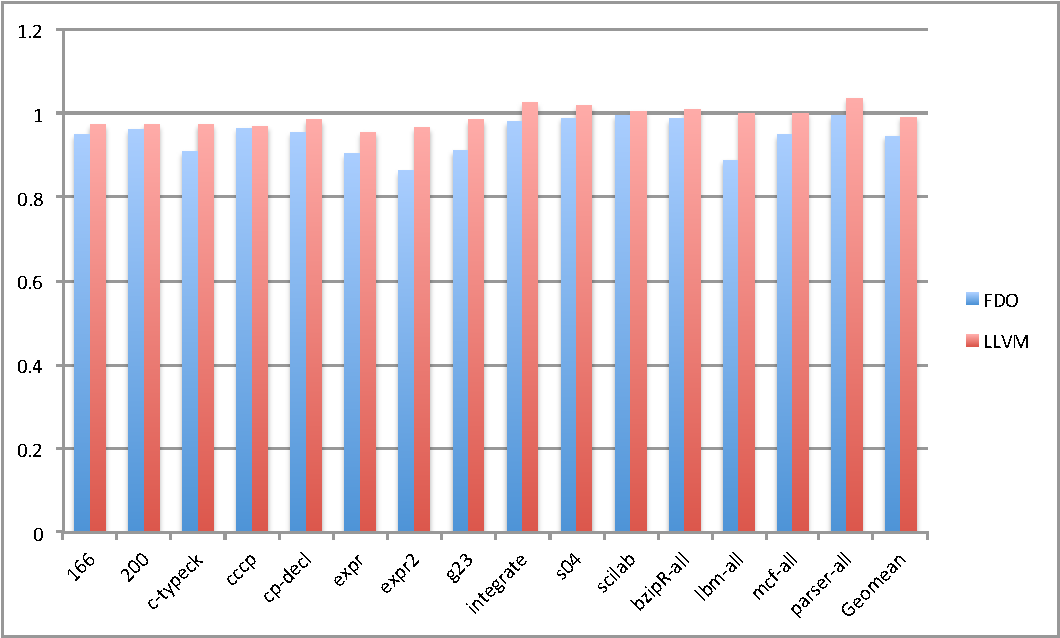
\includegraphics[width=0.4\linewidth]{Figures/speedupgccall}
     \label{fig:BestFDIWorstLLVMgcc}
  }
 \subfigure[\FDI\ is slower than \llvm;]{
    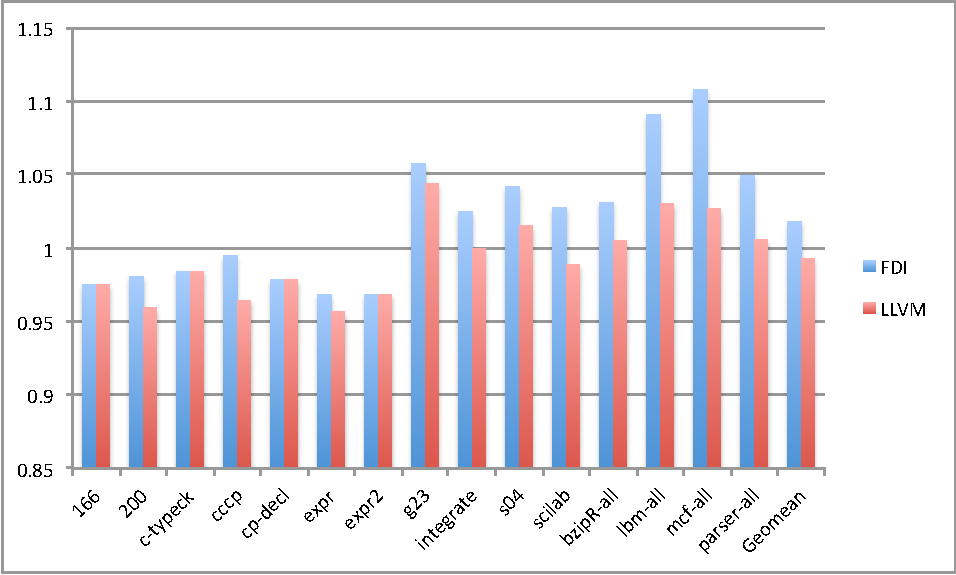
\includegraphics[width=0.4\linewidth]{Figures/slowdowngccall}
     \label{fig:BestFDIWorstLLVMgcc}
  }
  \end{center}
 \caption{Performance Study for \gcc. (a) Best runs of \FDI\ compared with worst runs of \llvm.  (b) Worst runs of \FDI\ compared with best runs of \llvm. Bar heights represent running time normalized to running time of Never}
  \label{fig:BestWorstComparison}
\end{figure*}
}
\REM{
\begin{center}$
\begin{array}{SS}
  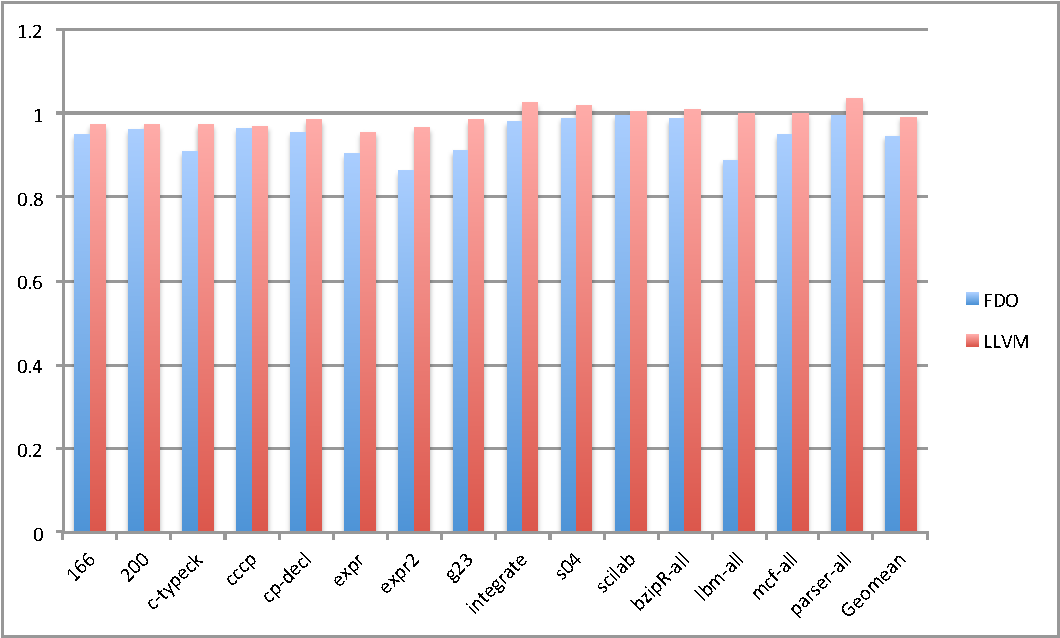
\includegraphics[width=0.5\linewidth]{Figures/speedupgccall} & 
  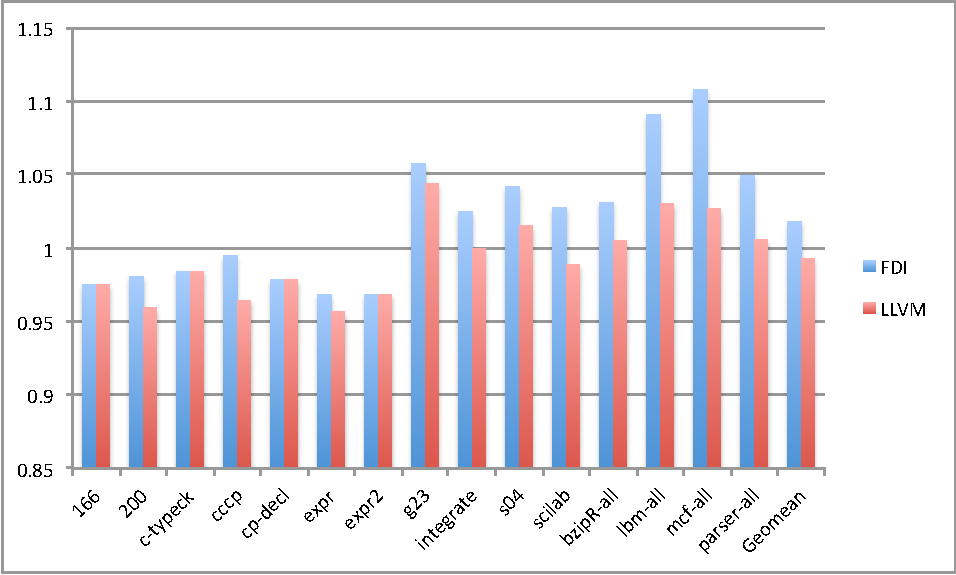
\includegraphics[width=0.5\linewidth]{Figures/slowdowngccall}\\
  \mathrm{(a) \FDI is faster than \llvm;} & \mathrm{(b) \FDI is slower than \llvm} \\
\end{array}$
 \begin{figure}
  \centering
    \caption{Running times of the slowdown measured for \gcc\ inlined versions, normalized by Never}
  \label{fig:slowdowngcc}
\end{figure}
}


\REM{
\subsection {Case Study 3: \gobmk}

For the case study with the SPEC CPU 2006 \gobmk, SPEC provides 20 inputs.  However, only 5 of these inputs come from the {\tt ref} workload; the {\tt train} workload contains 8 inputs, and the {\tt test} workload contains 7 inputs.  Many of the inputs from {\tt test} and {\tt train} have very short execution times: 4 inputs take less than 1 second, 6 take 2--9 seconds, 4 take 12--19 seconds, and 1 takes longer than 1 minute.  Execution times of less than a few seconds are subject to large proportional timing imprecision, because the Linux {\tt time} command reports times with a resolution of 1/100$^{th}$ of a second.  Therefore, the 15 longest-running inputs are chosen for \Wfull.  This set is composed of the {\tt ref} and {\tt train} SPEC workloads, plus \iname{connect} and \iname{dniwog} from {\tt test}.
}
%======== The inlining parameters

\REM{
As \FDI\ has a set of parameters that can vary and produce different running time for the programs, it was necessary to have a decision on the values for the set of parameter. These parameter values are the same through all benchmarks, and by using them the runtime results are quite similar to \llvm\ on average. That is why they were chosen, it is a very good parameter set for the purpose of this research.
}
%======= Reinforce the purpose

